The first step in integrating GPGPU-Sim into SST is to handle the interaction
with an SST CPU component. Since GPUs today function solely as co-processors,
functionally executing GPU-enabled binaries requires the CPU to initialize and
launch kernels of work to the GPU. In our model, the GPU is constructed out of
two types of discrete SST components -- a CTA scheduler and SM groups \cite{v100}.
When CUDA functions are called from the CPU component, they are intercepted and translated
into messages that are sent over SST links to the GPU (along with the associated
parameters). Table \ref{tab:apis} enumerates the CUDA API calls currently intercepted
and sent to the GPU components. These calls are enough to enable the execution of
a number of CUDA SDK kernels, DoE proxy apps as well as a collection of Kokkos Unit
tests. Table \ref{tab:kokkos_tests} lists the number of Kokkos unit tests that
pass with our current implementation of SST-GPU, which is about 60\%. There is
ongoing work with the PTX parser to increase the number of running kernels.


    \begin{table}[!htbp]
        \centering
        \setlength{\abovecaptionskip}{6pt plus 1pt minus 1pt}
        \captionsetup{width=.75\textwidth}
        \caption {CUDA API Calls Forwarded to the GPU components. Sched and SM represent CUDA calls
        sent to the scheduler or the SM groups. }
            \begin{tabular}{|l|c|c|}
                \hline
                CUDACall & Sched & SM \\
                \hline
                \hline
                \texttt{\textunderscore \textunderscore cudaRegisterFatBinary} & Yes & Yes \\
                \hline
                \texttt{\textunderscore \textunderscore cudaRegisterFunction} & Yes & Yes \\
                \hline
                \texttt{cudaMalloc} & Yes & No \\
                \hline
                \texttt{cudaMemcpy} & Yes & No \\
                \hline
                \texttt{cudaMemset} & Yes & No \\
                \hline
                \texttt{cudaConfigureCall} & Yes & Yes \\
                \hline
                \texttt{cudaSetupArgument} & Yes & Yes \\
                \hline
                \texttt{cudaFree} & Yes & No \\
                \hline
                \texttt{cudaLaunch} & Yes & Yes \\
                \hline
                \texttt{cudaGetLastError} & Yes & No \\
                \hline
                \texttt{cudaFuncSetCacheConfig} & Yes & No \\
                \hline
                \texttt{cudaSetDevice} & Yes & No \\
                \hline
                \texttt{cudaGetDeviceCount} & Yes & No \\
                \hline
                \texttt{cudaGetDeviceProperties} & Yes & No \\
                \hline
                \texttt{\textunderscore \textunderscore cudaRegisterVar} & Yes & Yes \\
                \hline
                \texttt{cudaOccupancyMaxActiveBlocksPerMultiprocessorWithFlags} & Yes & No \\
                \hline
            \end{tabular}
        \label{tab:apis}
    \end{table}


Aside from the basic functional model provided by GPU-SST, an initial
performance model has also been developed. Figure \ref{fig:gpu_sched} details
the overall architecture. A CPU component (Ariel in the initial implementation)
is connected via SST links to 2 types of GPU components: a centralized kernel and
CTA scheduler (GPUSched) and SM Groups, which implement the timing
and functional model for the GPU cores. When CUDA calls are intercepted
from the CPU, API commands are sent to the CTA scheduler. When the scheduler
launches a CTA for a kernel, CTA commands are sent to the corresponding SM groups
to execute. CUDA calls related to queuing kernels and memory operations are
handled by the scheduler, while execution related CUDA calls are redirect
to SM groups, since the functional model for executing the GPU CTAs lives inside
the SM groups. Table \ref{tab:apis} shows where CUDA calls send to. 

   \begin{figure}[!htb]
      \centering
      \setlength{\abovecaptionskip}{6pt plus 1pt minus 1pt}
      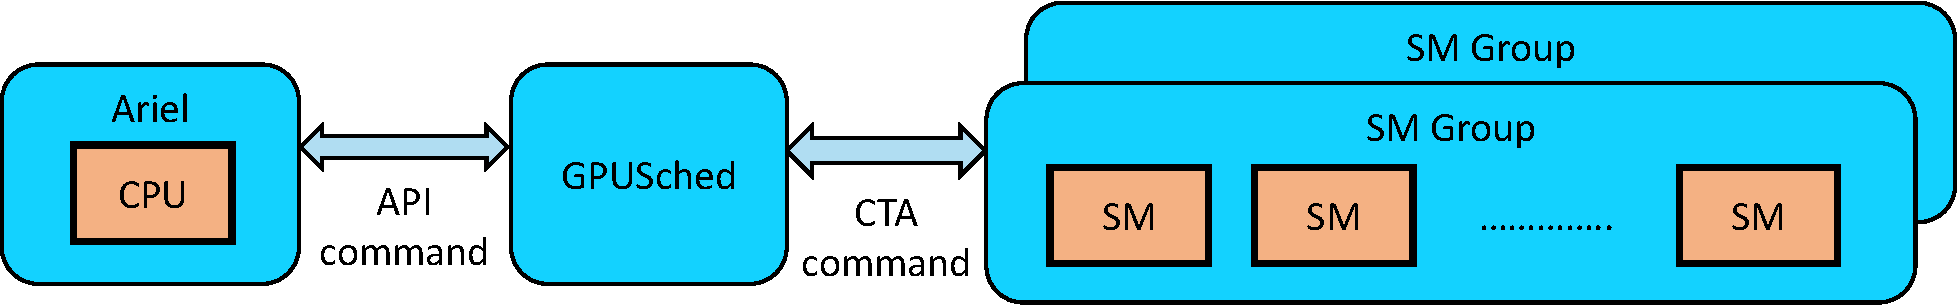
\includegraphics[width=.90\textwidth,keepaspectratio]{figures/2_1-eps-converted-to-crop.pdf}
      \captionsetup{width=.90\textwidth}
      \caption{SST component architecture for CTA scheduler and SM groups}
      \label{fig:gpu_sched}
   \end{figure}


As CTAs complete on the SMs, commands are sent back to the GPU scheduler
component, which pushes new work to the SMs from enqueued kernels as needed.
Memory copies from the CPU to GPU address space are handled on a configurable
page-size granularity, similar to how conventional CUDA unified memory handles
the transfer of data from CPU to GPU memories.

   \begin{figure}[!htb]
      \centering
      \setlength{\abovecaptionskip}{6pt plus 1pt minus 1pt}
      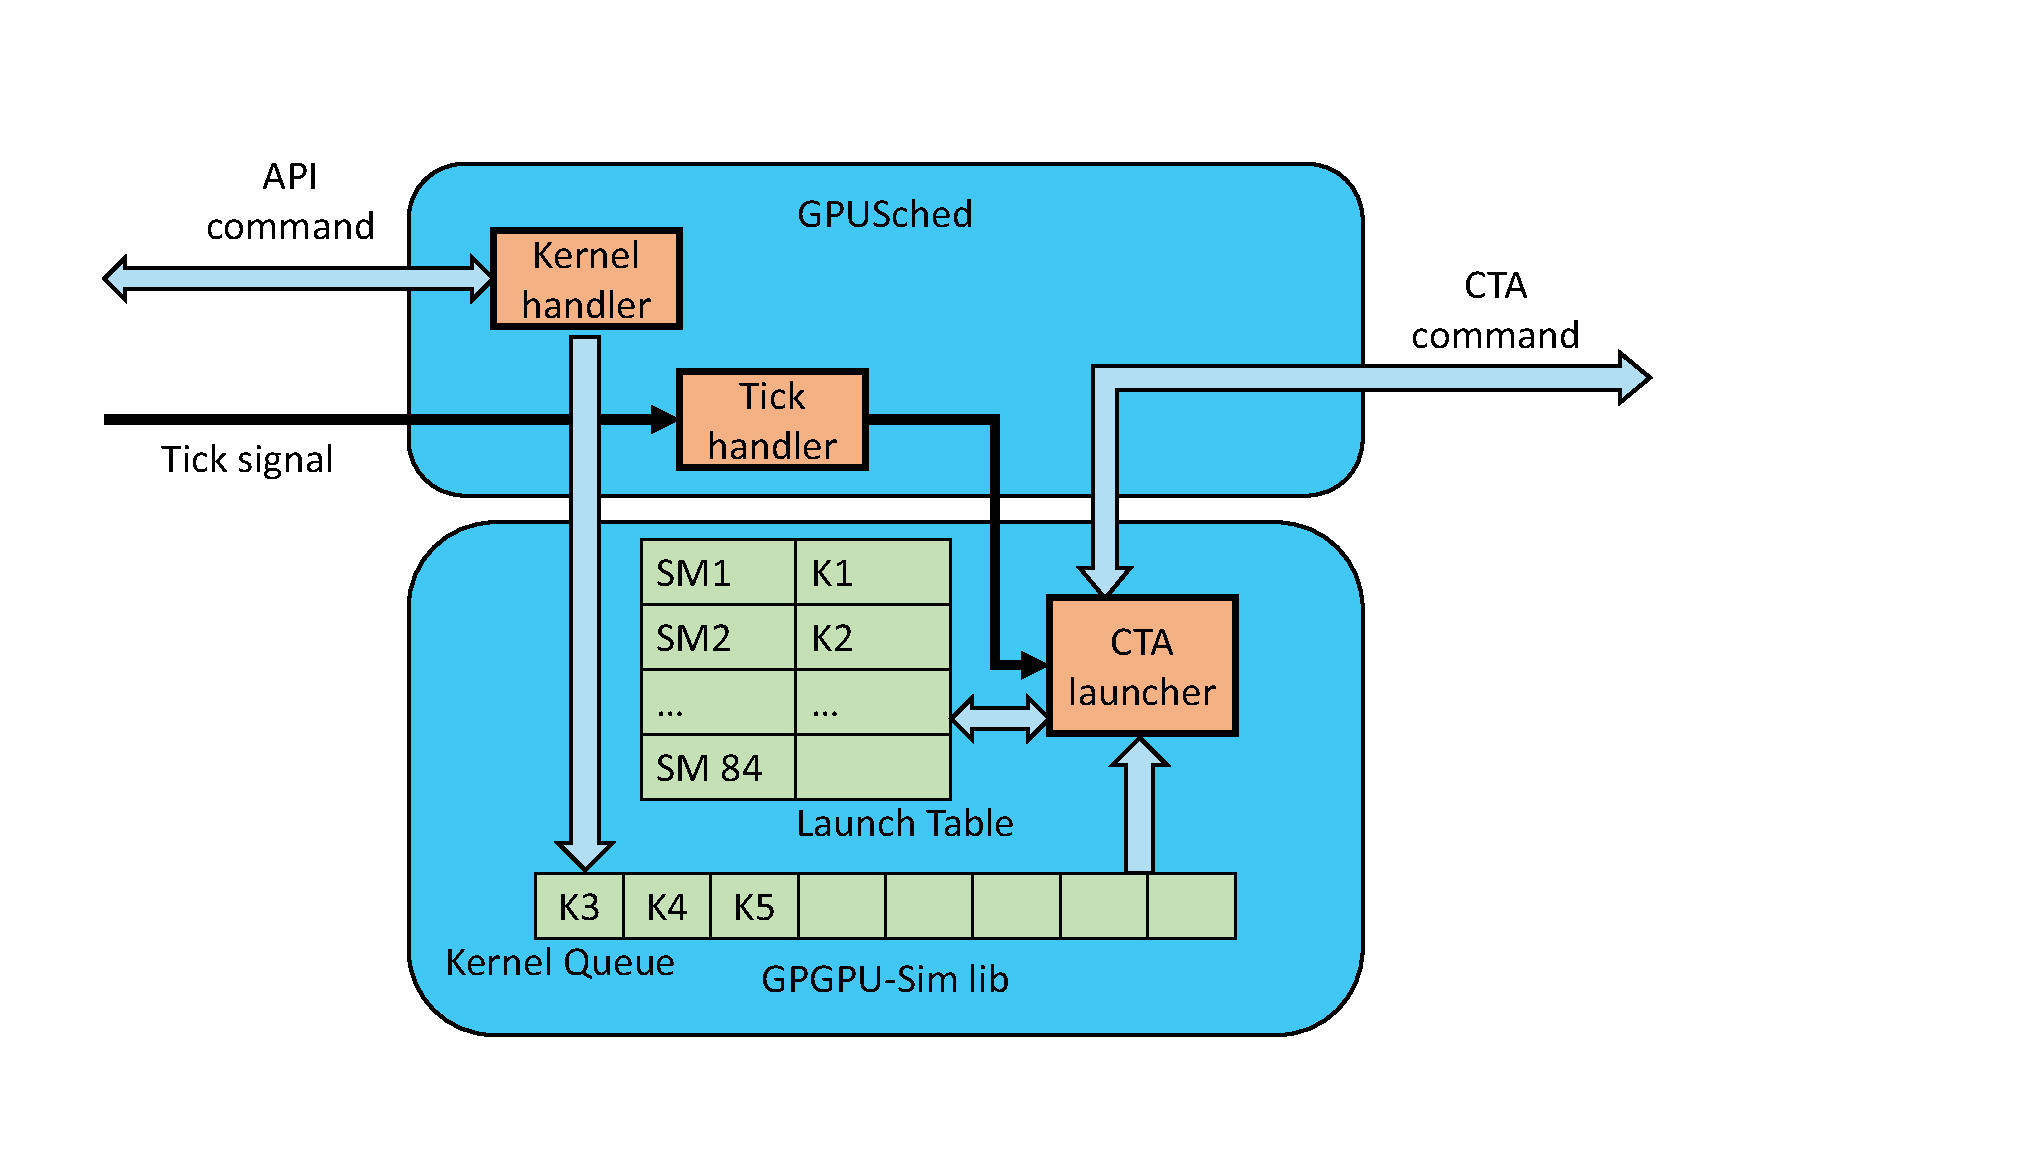
\includegraphics[width=.90\textwidth,keepaspectratio]{figures/scheduler.eps}
      \captionsetup{width=.75\textwidth}
      \caption{Centralized GPU scheduler component}
      \label{fig:sched}
   \end{figure}

The centralized GPU scheduler receives kernel launch commands from the CPU, then
issues CTA launch commands to the SMs. The scheduler also receives notifications
from the SMs when the CTAs finish. The reception of kernel launch and CTA
complete notifications are independent, therefore we designed a different
handler for each type of message. Figure~\ref{fig:sched} shows the design of the
centralized kernel and CTA Scheduler. The kernel handler listens to calls from a
CPU component and pushes kernel launch information to the kernel queue when it
receives kernel configure and launch commands. The SM launch table contains CTA
slots for each of the SMs, which is reserved when launching a CTA and released when a
message indicating that a CTA has finished is received from the SMs. The
scheduler clock ticks trigger CTA launches to SMs, when space is available and
there is a pending kernel. On every tick, the scheduler issues a CTA launch
command for currently unfinished kernels if any CTA slot is available or tries
to fetch a new kernel launch from kernel queue. The CTA handler also waits for
SMs to reply the CTA finish message, so that CTA slots in the SM launch table may
be freed.
